\documentclass{article}

\usepackage{siunitx} % Provides the \SI{}{} and \si{} command for typesetting SI units
\usepackage{graphicx} % Required for the inclusion of images
\usepackage{amsmath} % Required for some math elements 
\usepackage[export]{adjustbox} % loads also graphicx
\usepackage{listings}
\usepackage{matlab-prettifier}
\usepackage{float}
\usepackage[most]{tcolorbox}
\usepackage{amsfonts}
\usepackage{color}
\usepackage{titlesec}
\usepackage{caption}
\usepackage{subcaption}
\usepackage{placeins}

\newcommand{\R}{\mathbb{R}}

\usepackage{xcolor}

\DeclareCaptionFont{white}{\color{white}}
\DeclareCaptionFormat{listing}{%
  \parbox{\textwidth}{\colorbox{gray}{\parbox{\textwidth}{#1#2#3}}\vskip-4pt}}
\captionsetup[lstlisting]{format=listing,labelfont=white,textfont=white}
\lstset{frame=lrb,xleftmargin=\fboxsep,xrightmargin=-\fboxsep}
\titleformat{\section}[runin]
  {\normalfont\Large\bfseries}{\thesection}{1em}{}
\titleformat{\subsection}[runin]
  {\normalfont\large\bfseries}{\thesubsection}{1em}{}


\setlength\parindent{0pt} % Removes all indentation from paragraphs

\renewcommand{\labelenumi}{\alph{enumi}.} % Make numbering in the enumerate environment by letter rather than number (e.g. section 6)

%\usepackage{times} % Uncomment to use the Times New Roman font

%----------------------------------------------------------------------------------------
%	DOCUMENT INFORMATION
%----------------------------------------------------------------------------------------

\title{AMATH 353: Homework 14 \\Due May, 30 2018 \\ ID: 1064712} % Title

\author{Trent \textsc{Yarosevich}} % Author name

\date{\today} % Date for the report

\begin{document}
\maketitle % Insert the title, author and date
\setlength\parindent{1cm}

\begin{center}
\begin{tabular}{l r}
%Date Performed: December 1, 2017 \\ % Date the experiment was performed
Instructor: Jeremy Upsal % Instructor/supervisor
\end{tabular}
\end{center}

% If you wish to include an abstract, uncomment the lines below
% \begin{abstract}
% Abstract text
% \end{abstract}

%----------------------------------------------------------------------------------------
%	SECTION 1
%----------------------------------------------------------------------------------------
\section*{Part 1}
\subsection*{(a)}
Given the following initial condition, we get:
\begin{equation}
u(x,0)= 
  \begin{cases}
			\frac{\pi}{2}, \; \; \; x < 1 \\
			\frac{\pi}{4}, \; \; \; x \geq 1 \\
            \end{cases}
\
\end{equation}
\begin{equation}
\begin{aligned}
\frac{du}{dt} = 0\\
u(x(t), t) = A\\
A = u_0(x_0) = u(x, 0)\\
\end{aligned}
\end{equation}
We can then make use of $x(t) = x_0 + c(u_0(x_0)t$: and determine the equations for the characteristics:
\begin{equation}
\begin{aligned}
c(u(x(t), t)) = \sin(u)\\
c(u_0(x_0) = \sin(u_0(x_0))\\
\end{aligned}
\end{equation}
\begin{equation}
c(u_0(x_0) 
  \begin{cases}
			1, \; \; \; x_0 < 1 \\
			\frac{\sqrt{2}}{2}, \; \; \; x_0 \geq 1 \\
            \end{cases}
\
\end{equation}
This in turn gives the following characteristics curves:
\begin{equation}
x(t) = 
  \begin{cases}
			x_0 + t, \; \; \; x_0 < 1 \\
			x_0 + \frac{\sqrt{2}}{2}t, \; \; \; x_0 \geq 1 \\
            \end{cases}
\
\end{equation}
\begin{equation}
t = 
  \begin{cases}
			x - x_0, \; \; \; x_0 < 1 \\
			\sqrt{2}(x - x_0) \; \; \; x_0 \geq 1 \\
            \end{cases}
\
\end{equation}
Additionally, here are the functions of $x_0$ in terms of $x$ and $t$, which will be useful later:
\begin{equation}
x_0 =
  \begin{cases}
			x - t, \; \; \; x_0 < 1 \\
			x - \frac{\sqrt{2}}{2}t \; \; \; x_0 \geq 1 \\
            \end{cases}
\
\end{equation}
\subsection*{(b)}
%Also have to show that the slope to the left of the discontinuity are greater than those to the left.

Because $u(x(t), t) = u_0(x_0)$ we can find the breaking time by finding where its derivative goes to $\infty$. 
\begin{equation}
u_x = u_0'(x_0)\frac{dx_0}{dx}\\
\end{equation}
It is clear from the initial condition given above that we cannot take the derivative $u_0'(x_0)$ because $u_0(x_0)$ has a discontinuity when $x_0 = 1$. Plugging this into equation (7) above at $t=0$ we see that this occurs at $x = 1$.
\subsection*{(c)}
Since $\phi(x,t) = \sin(u)u_x$ we can integrate to get the following (note that I am ignoring the constant of integration, since it drops out in the Rankine-Hugoniot relation anyway):
\begin{equation}
\phi(x, t) = -\cos(u)
\end{equation}
We know from equation (2) above that $u^- = \frac{\pi}{2}$ and $u^+ = \frac{\pi}{4}$ giving:
\begin{equation}
\begin{aligned}
\frac{dx_s}{dt} = \frac{[\phi]}{[u]}\\
\frac{[\phi]}{[u]} = \frac{-\cos(u^+) + \cos(u^-)}{u^+ - u^-}\\
\frac{dx_s}{dt} = \frac{-\frac{\sqrt{2}}{2}}{-\frac{\pi}{4}}
\end{aligned}
\end{equation}
Which simplifies to:
\begin{equation}
\frac{dx_s}{dt} = \frac{2\sqrt{2}}{\pi}
\end{equation}
We then integrate and apply the initial condition found in (b):
\begin{tcolorbox}[minipage,colback=white,arc=0pt,outer arc=0pt]
\begin{equation}
\begin{aligned}
x_s(t) = \frac{2\sqrt{2}}{\pi}t + C\\
x_s(0) = 1 = C\\
x_s(t) = \frac{2\sqrt{2}}{\pi}t + 1
\end{aligned}
\end{equation}
\end{tcolorbox}
\begin{figure}[!htbp]
  \centering
    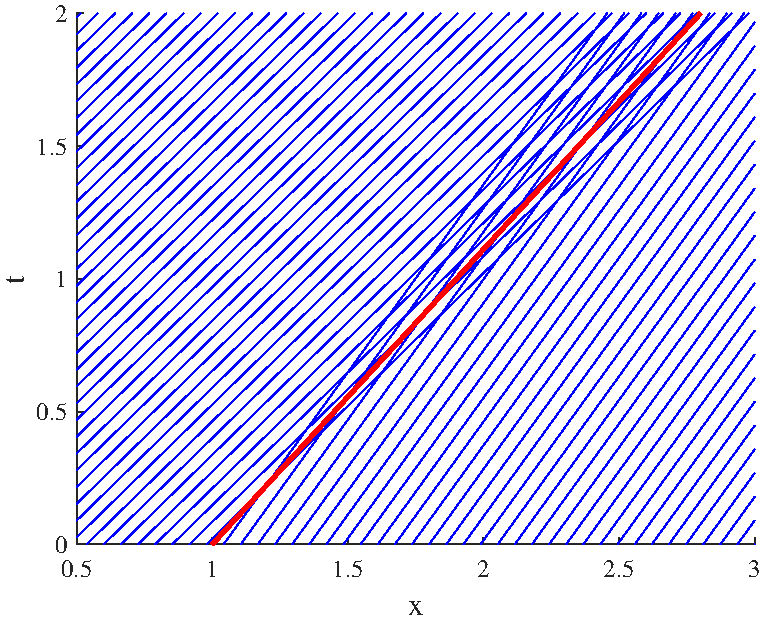
\includegraphics[width=\textwidth]{hw_14_plot1.pdf}
    \caption{Characteristics and $x_s$}
\end{figure}
\FloatBarrier
\subsection*{(d)}
The solution to the left of the shockline is a line at $u = \frac{\pi}{2}$, and to the right, a line at $u = \frac{\pi}{4}$. This is defined as: 
\begin{tcolorbox}[minipage,colback=white,arc=0pt,outer arc=0pt]
\begin{equation}
u(x,t) =
  \begin{cases}
			\frac{\pi}{2}, \; \; \; x < x_s \\
			\frac{\pi}{4} \; \; \; x \geq x_s \\
            \end{cases}
\
\end{equation}
\end{tcolorbox}
\subsection*{(e)}
If we change the characteristics in this way, the speed in the $u^+$ region is actually greater than it is in the $u^-$. As a result, the space between the solutions for $u$ actually increases in time, giving a growing region in which $u$ is not defined. 
\begin{figure}[!htbp]
  \centering
    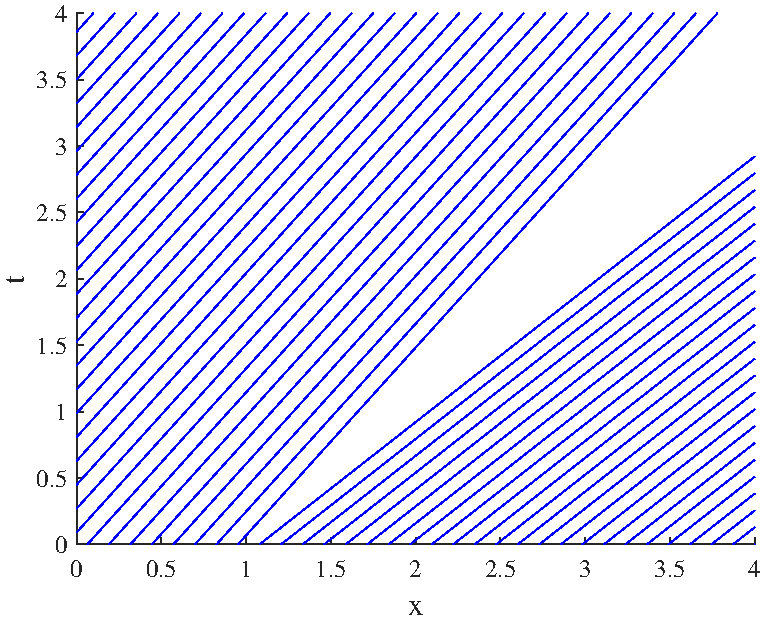
\includegraphics[width=\textwidth]{hw_14_plot2.pdf}
    \caption{$u^-=\frac{\pi}{4}$ and $u^+=\frac{\pi}{2}$}
\end{figure}
\FloatBarrier
\section*{Part 2}
\subsection*{(a)}
\begin{figure}[!htbp]
  \centering
    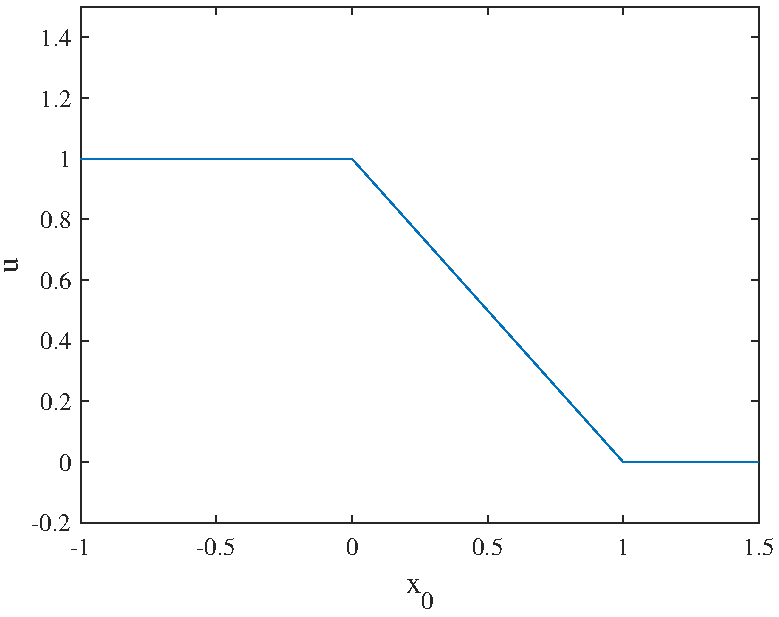
\includegraphics[width=\textwidth]{hw_14_plot3.pdf}
    \caption{$u(x, 0)$}
\end{figure}
\FloatBarrier
\subsection*{(b)}
First, we obtain the solution to $u$ along the characteristics:
\begin{equation}
\begin{aligned}
\frac{du}{dt} = 0\\
u(x(t), t) = A\\
A = u(x,0) = u_0(x_0)\\
\end{aligned}
\end{equation}
\begin{equation}
u(x(t),t) =
  \begin{cases}
			1, \; \; \; x_0 \leq 0 \\
			1-x_0, \; \; \; 0 < x_0 < 1\\
			0, \; \; \; x_0 \geq 1\\
            \end{cases}
\
\end{equation}
Using the values for $u_0(x_0)$ and $x(t) = x_0 + c(u_0(x_0))t$, we then obtain the characteristic curves:
\begin{tcolorbox}[minipage,colback=white,arc=0pt,outer arc=0pt]
\begin{equation}
x(t) =
  \begin{cases}
			x_0 + t, \; \; \; x_0 \leq 0 \\
			x_0 + t(1-x_0), \; \; \; 0 < x_0 < 1\\
			x_0, \; \; \; x_0 \geq 1\\
            \end{cases}
\
\end{equation}
\end{tcolorbox}
\subsection*{(c)}
We know from Knobel's that a solution for $u(x,t)$ when a shock forms must have continuous first derivatives in the regions to the left and right of the shock line. When we take the derivative $u'_0(x_0)$ from equaton (15) we have the following:
\begin{equation}
u'_0(x_0) =
  \begin{cases}
			0, \; \; \; x_0 \leq 0 \\
			-1, \; \; \; 0 < x_0 < 1\\
			0, \; \; \; x_0 \geq 1\\
            \end{cases}
\
\end{equation}
This derivative is discontinuous at $x_0 = 0, 1$ and so no two regions exist such that there would be continuous derivatives on each side. However, we can deduce a few things looking at the speed of the initial profile, which is equal to $u$. The value of $u$ when $x_0 <0$ is 1, so it is moving to the right, and the value when $x \geq 1$ is 0, so it is not moving in time. The middle region's value from $0<x<1$ is $1-x_0$ so the top of the profile is moving faster than the bottom, so over time it will form a vertical line as $x_0$ approaches 1. This means that if these characteristic lines at $x_0 = 0, 1$ intersect, there will be smooth first derivatives on each side, and furthermore there will be an jump in the solutions, and thus a shockwave. Plugging these values of $x_0$ into equation (16) we get:
\begin{tcolorbox}[minipage,colback=white,arc=0pt,outer arc=0pt]
\begin{equation}
\begin{aligned}
x_0 = 0 = x -t\\
x_0 = 1 = x\\
0 = 1 - t\\
t_b = 1
\end{aligned}
\end{equation}
\end{tcolorbox}
\subsection*{(d)}
Using equation (16) above, we can solve for $x_0$ for each of the 3 ranges. $x_0 \leq 0$ and $x_0 \geq 0$ are fairly straightforward, so I won't show my work for those. For $0 < x_0 < 1$ however, we have the following:
\begin{equation}
\begin{aligned}
x(t) = x_0 + t(1-x_0)\\
\frac{x}{x_0} = 1 - t + \frac{t}{x_0}\\
\frac{x}{x_0} - \frac{t}{x_0} = 1 - t\\
\frac{1}{x_0}(x - t) = 1 -t\\
x_0 = \frac{x -t}{1-t}
\end{aligned}
\end{equation}
We then have:
\begin{equation}
x_0 =
  \begin{cases}
			x - t, \; \; \; x_0 \leq 0 \\
			\frac{x -t}{1-t}, \; \; \; 0 < x_0 < 1\\
			x, \; \; \; x_0 \geq 1\\
            \end{cases}
\
\end{equation}
We can then substitute these values into equation (16) to obtain the solution for $t < t_b$. Again, the substitutions are fairly straightforward, but I will show the work for $0 < x_0 < 1$.
\begin{equation}
\begin{aligned}
0 < \frac{x -t}{1-t} < 1\\
0 < x - t < 1 - t\\
t < x < 1
\end{aligned}
\end{equation}
And finally substituting all this into (15) gives the solution for $0 \leq t < t_b$. We can see in this solution that the middle constraint solutions only exist in a range between $t=0$, $x = 1$ and $t = x$, as described in part (c).
\begin{tcolorbox}[minipage,colback=white,arc=0pt,outer arc=0pt]
\begin{equation}
u(x,t) = 
  \begin{cases}
			1, \; \; \; x \leq t \\
			1-\frac{x -t}{1-t}, \; \; \; t < x < 1\\
			0, \; \; \; x \geq 1\\
            \end{cases}
\
\end{equation}
\end{tcolorbox}
\subsection*{(e)}
We can see from the stated problem that $\phi_x = uu_x$. Integrating this gives
\begin{equation}
\phi = \frac{u^2}{2}
\end{equation}
Considering equation (22) above, we can see that at the breaking time $t_b = 1$, the solution is defined in two regions as the second constraint $t < x < 1$ is not satisfied for any $t > t_b = 1$. This leaves the other two constraints:
\begin{equation}
\begin{aligned}
u^- = 1, \; x < t\\
u^+ = 0, \; x \geq 1
\end{aligned}
\end{equation}
With this information we can then use the Rankine-Hugoniot relation:
\begin{equation}
\begin{aligned}
\frac{dx_0}{dt} = \frac{\frac{0^2}{2} - \frac{1^2}{2}}{0 - 1}\\
\frac{dx_0}{dt} = \frac{1}{2}\\
x_s(t) = \frac{1}{2}t + C\\
x_s(1) = 1  = \frac{1}{2}(1) + C\\
x_s(t) = \frac{1}{2}t + \frac{1}{2}
\end{aligned}
\end{equation}
\subsection*{(f)}
Making use equations (22), (24), and (25) above:
\begin{equation}
  u(x,t)=
  \begin{cases}
    \begin{cases}
      1, & x \leq t \\
      1 - \frac{x-t}{1-t}, & t < x < 1\\
      0, & x \geq 1
    \end{cases}
    &0 < t < 1\\
    \begin{cases}
      1,  & x < x_s(t) \\
      0,  & x > x_s(t)
    \end{cases}
    &t\geq 1
  \end{cases}
\end{equation}
\subsection*{(g)}
\begin{figure}[H]
  \centering
  \begin{minipage}[b]{0.49\textwidth}
    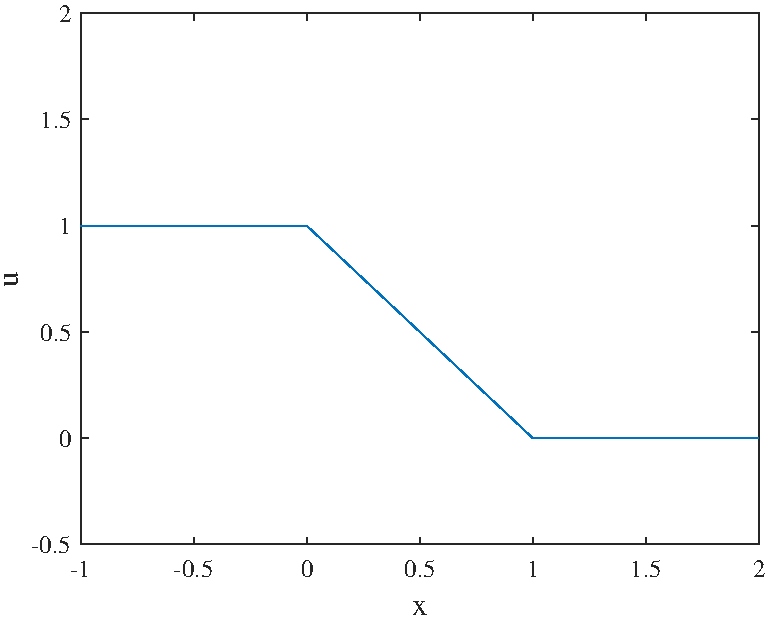
\includegraphics[width=\textwidth]{hw_14_plot5.pdf}
    \caption{$t = 0$}

  \end{minipage}
  \hfill
  \begin{minipage}[b]{0.49\textwidth}
    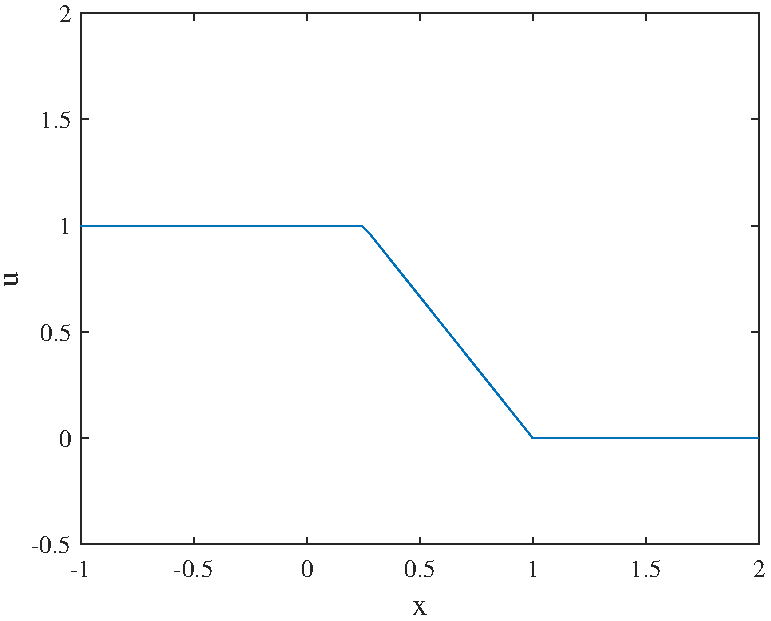
\includegraphics[width=\textwidth]{hw_14_plot6.pdf}
    \caption{$t = 0.25$}

  \end{minipage}
    \hfill
  \begin{minipage}[b]{0.49\textwidth}
    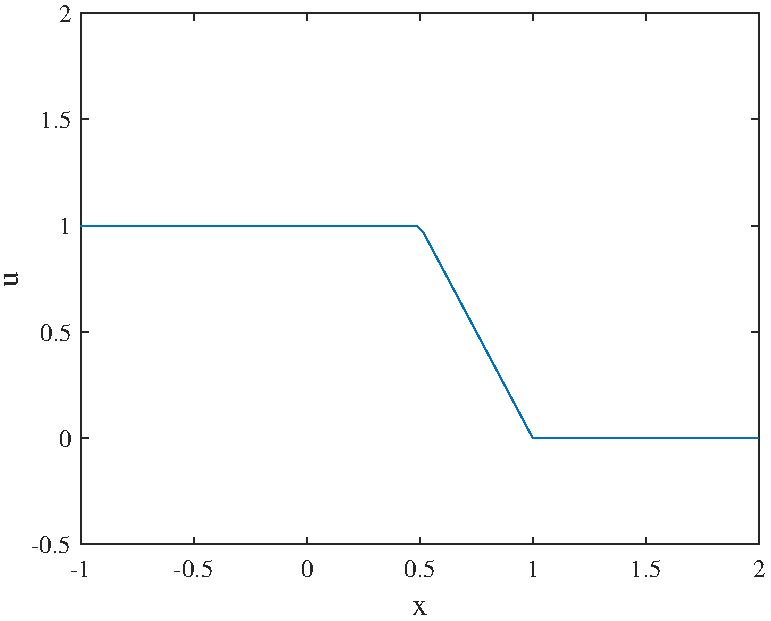
\includegraphics[width=\textwidth]{hw_14_plot7.pdf}
    \caption{$t = 0.5$}

  \end{minipage}
    \hfill
  \begin{minipage}[b]{0.49\textwidth}
    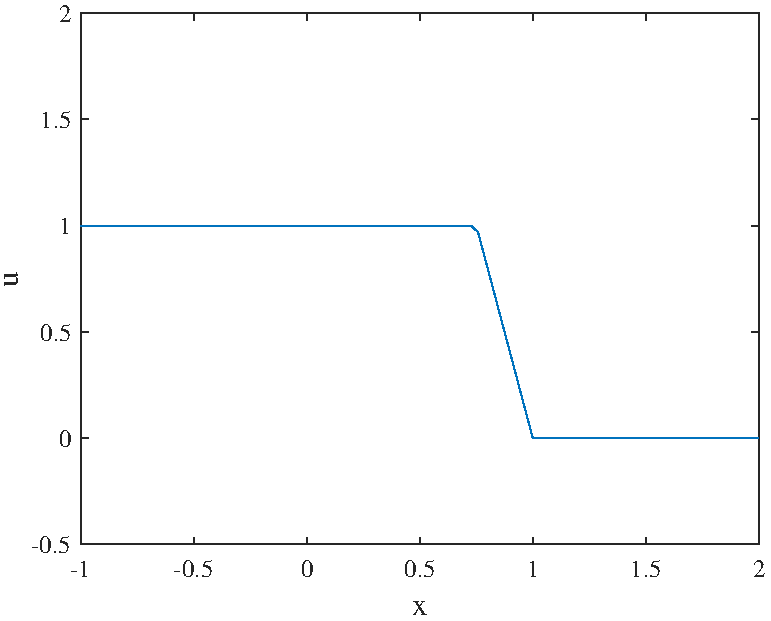
\includegraphics[width=\textwidth]{hw_14_plot8.pdf}
    \caption{$t = .75$}

  \end{minipage}
      \hfill
  \begin{minipage}[b]{0.49\textwidth}
    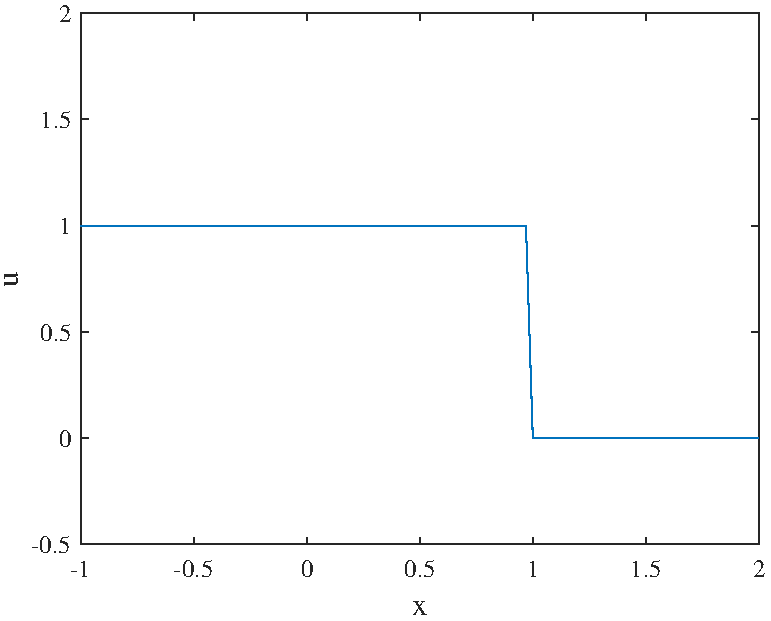
\includegraphics[width=\textwidth]{hw_14_plot9.pdf}
    \caption{$t = 1$}

  \end{minipage}
      \hfill
  \begin{minipage}[b]{0.49\textwidth}
    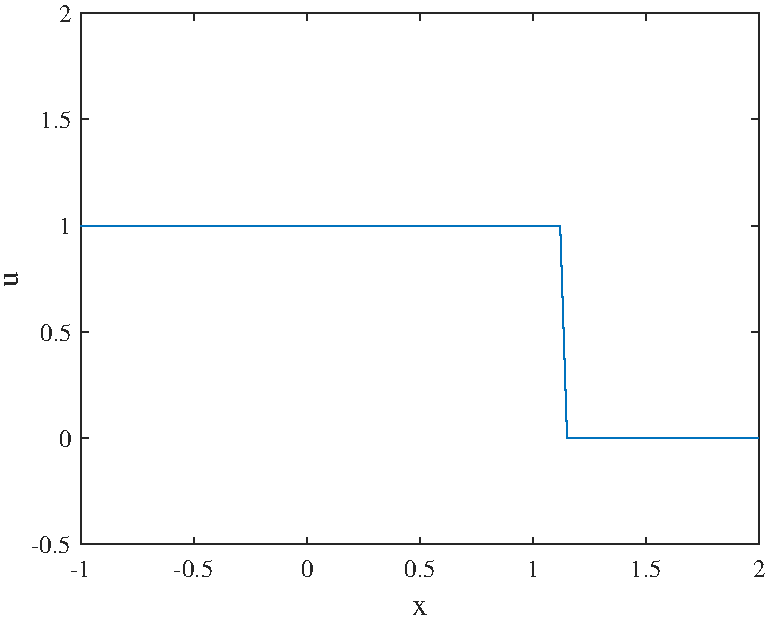
\includegraphics[width=\textwidth]{hw_14_plot10.pdf}
    \caption{$t = 1.25$}

  \end{minipage}
    \hfill
  \begin{minipage}[b]{0.49\textwidth}
    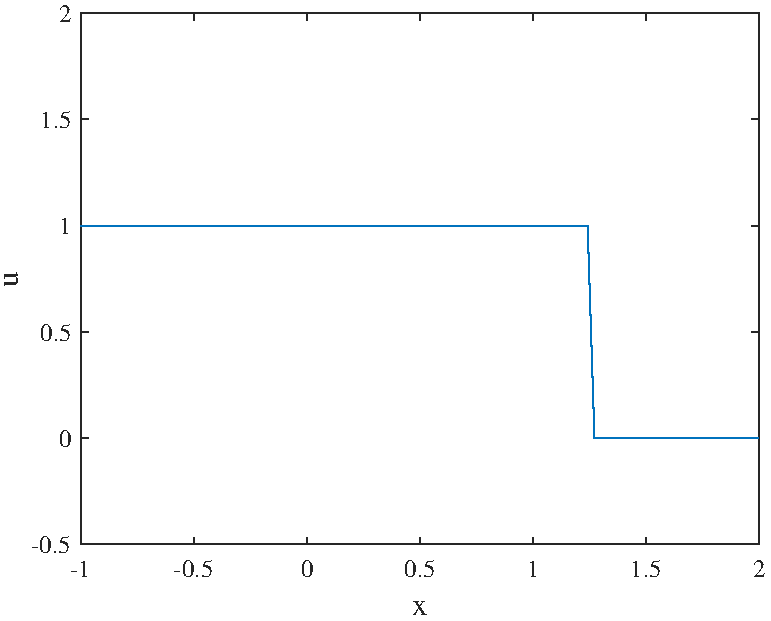
\includegraphics[width=\textwidth]{hw_14_plot11.pdf}
    \caption{$t = 1.5$}

  \end{minipage}
      \hfill
  \begin{minipage}[b]{0.49\textwidth}
    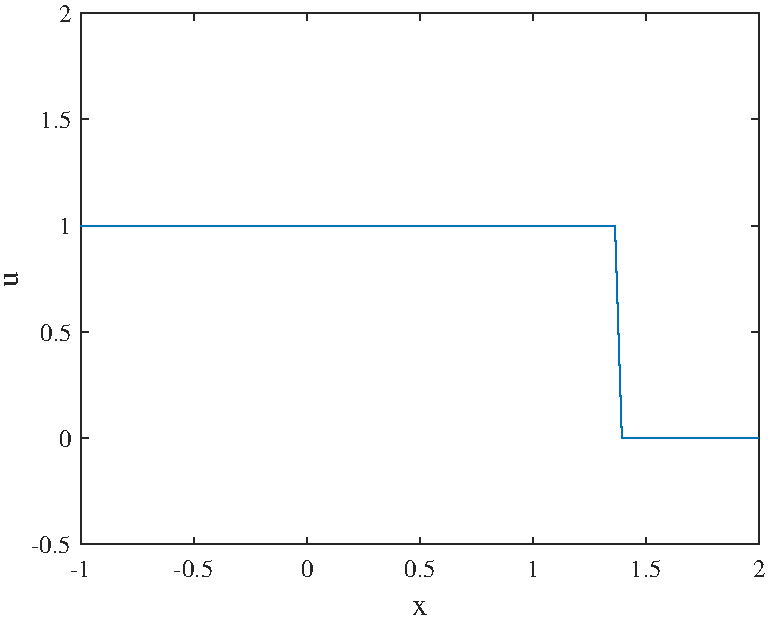
\includegraphics[width=\textwidth]{hw_14_plot12.pdf}
    \caption{$t = 1.75$}

  \end{minipage}
\end{figure}
\begin{figure}[!htbp]
  \centering
    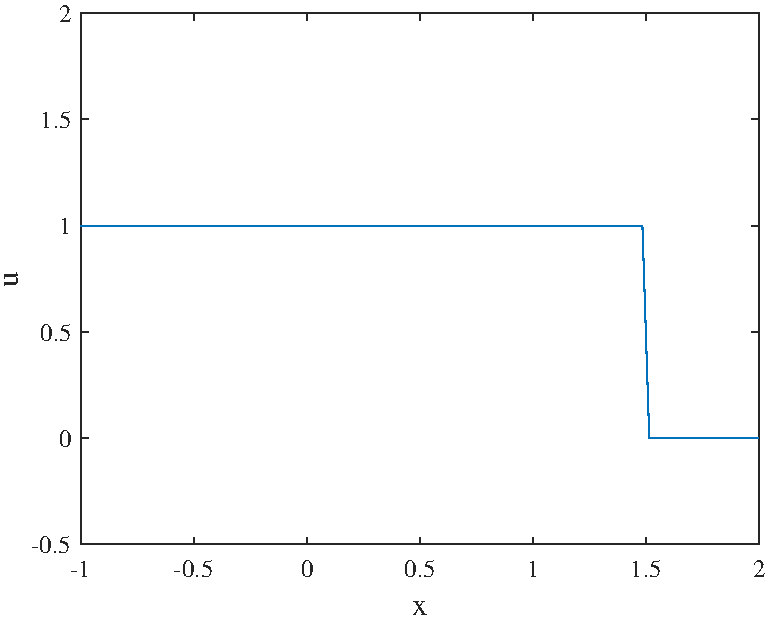
\includegraphics[width=.49\textwidth]{hw_14_plot13.pdf}
    \caption{$t = 2$}
\end{figure}
\section*{Part 3}
\subsection*{(a)}
For these values, there is no change in density of cars at any point, thus no shock/traffic jam forms. Information travels forward at a uniform speed of $v = v_1(1 - \frac{\frac{u_1}{3}}{u_1}) = \frac{2}{3}v_1$. NOTE THIS IS WRONG IT'S JUST THE RELATION
\begin{figure}[!htbp]
  \centering
    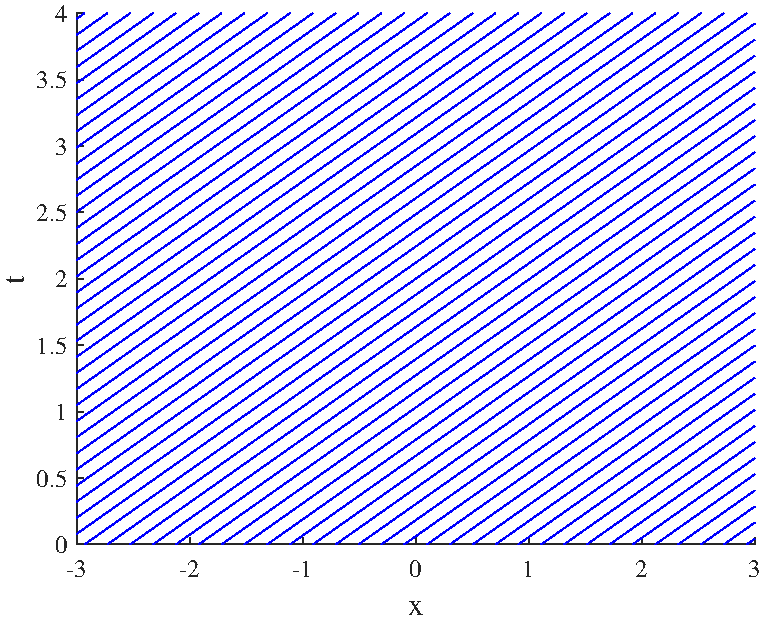
\includegraphics[width=.49\textwidth]{hw_14_plot14.pdf}
    \caption{}
\end{figure}
\subsection*{(b)}
%shwo the slope of the shock line in order to demonstrate that the information is moving forward.

For these values a traffic jam forms immediately at $t=0$. If you zoom in on the graph, it's clear that information is traveling forward, which is also clear since the $u^+$ value is less than $u_1$. Overall this means traffic hits the traffic jam and then immediately slows to a much lower speed. 
\begin{figure}[!htbp]
  \centering
    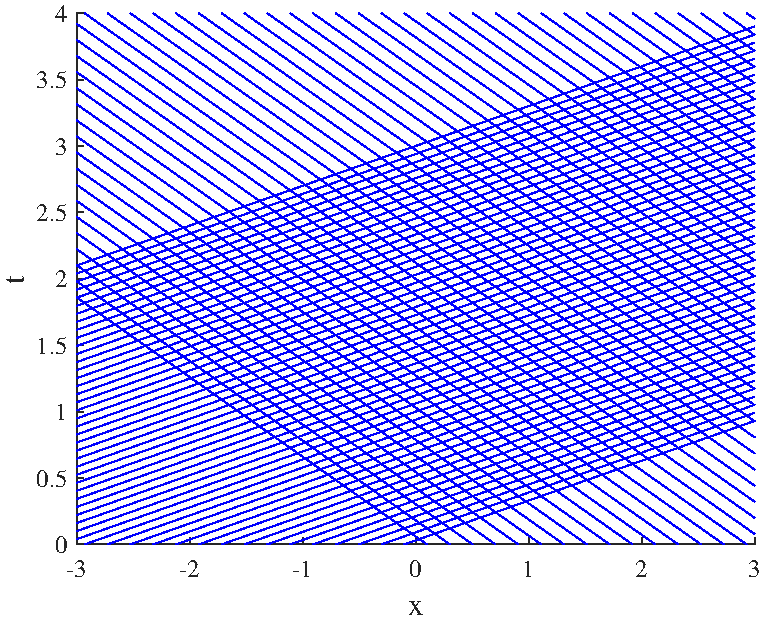
\includegraphics[width=.49\textwidth]{hw_14_plot15.pdf}
    \caption{}
\end{figure}
\FloatBarrier

\subsection*{(c)}
For these values, traffic is moving more slowly on the left and more quickly on the right, and thus a region forms in which there are no characteristics, and thus no solution to $u$. Intuitively, this would seem to model an area in which there are no cars because two 'packs' of cars are getting further and further apart. As to why this would happen, I can think of a few scenarios, but some, like a change in speed limit, mess with our model. Perhaps an area in which a single lane opens up to two lanes, but this wouldn't explain the widening region in which $u$ is undefined.
\begin{figure}[!htbp]
  \centering
    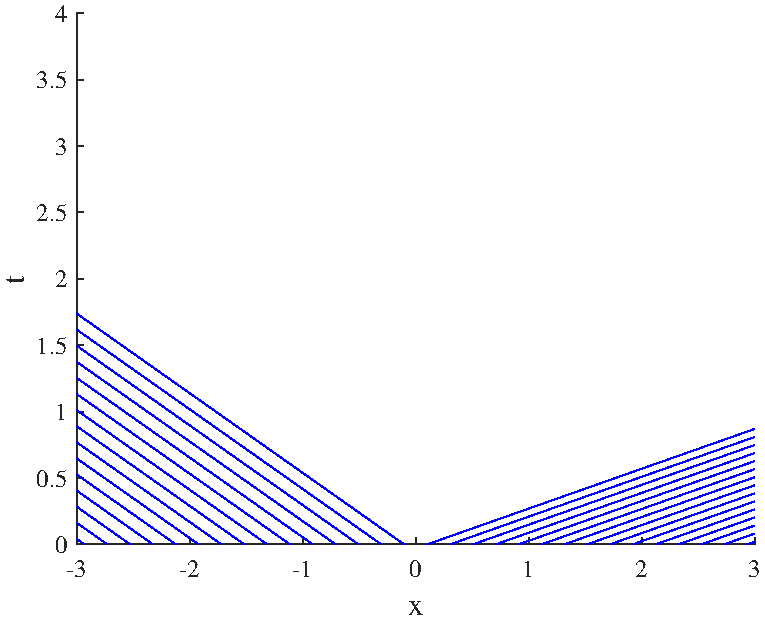
\includegraphics[width=.49\textwidth]{hw_14_plot16.pdf}
    \caption{}
\end{figure}
\FloatBarrier
\subsection*{(d)}
% also need to observe that both slopes need to have the same sign in order for shocks to form.

The slope of the characteristics in the traffic problem are give by 
\begin{equation}
\frac{1}{v_1(1-\frac{2u^{\pm}}{u_1})}
\end{equation}
We can see that when the slope of the characteristics in the left region are greater than the ones in the right, they will cross (regardless of whether the slopes are positive or negative). We then have:
\begin{equation}
\frac{1}{v_1(1-\frac{2u^-}{u_1})} \geq \frac{1}{v_1(1-\frac{2u^+}{u_1})}
\end{equation}
This then very quickly simplifies down to $u^- \geq u^+$, which is to say if the initial density is higher on the left than it is on the right, no shock will form.
\end{document}
